In particolare, il Diagramma delle Classi (\textit{Class Diagram}) definisce l'architettura statica del software secondo i paradigmi della \textit{programmazione Object-Oriented (OOP)}. All'interno di tale diagramma vengono strutturate le classi relative alla gestione dei vari profili d'accesso presenti nel sistema.
\begin{figure}[H]
    \centering
    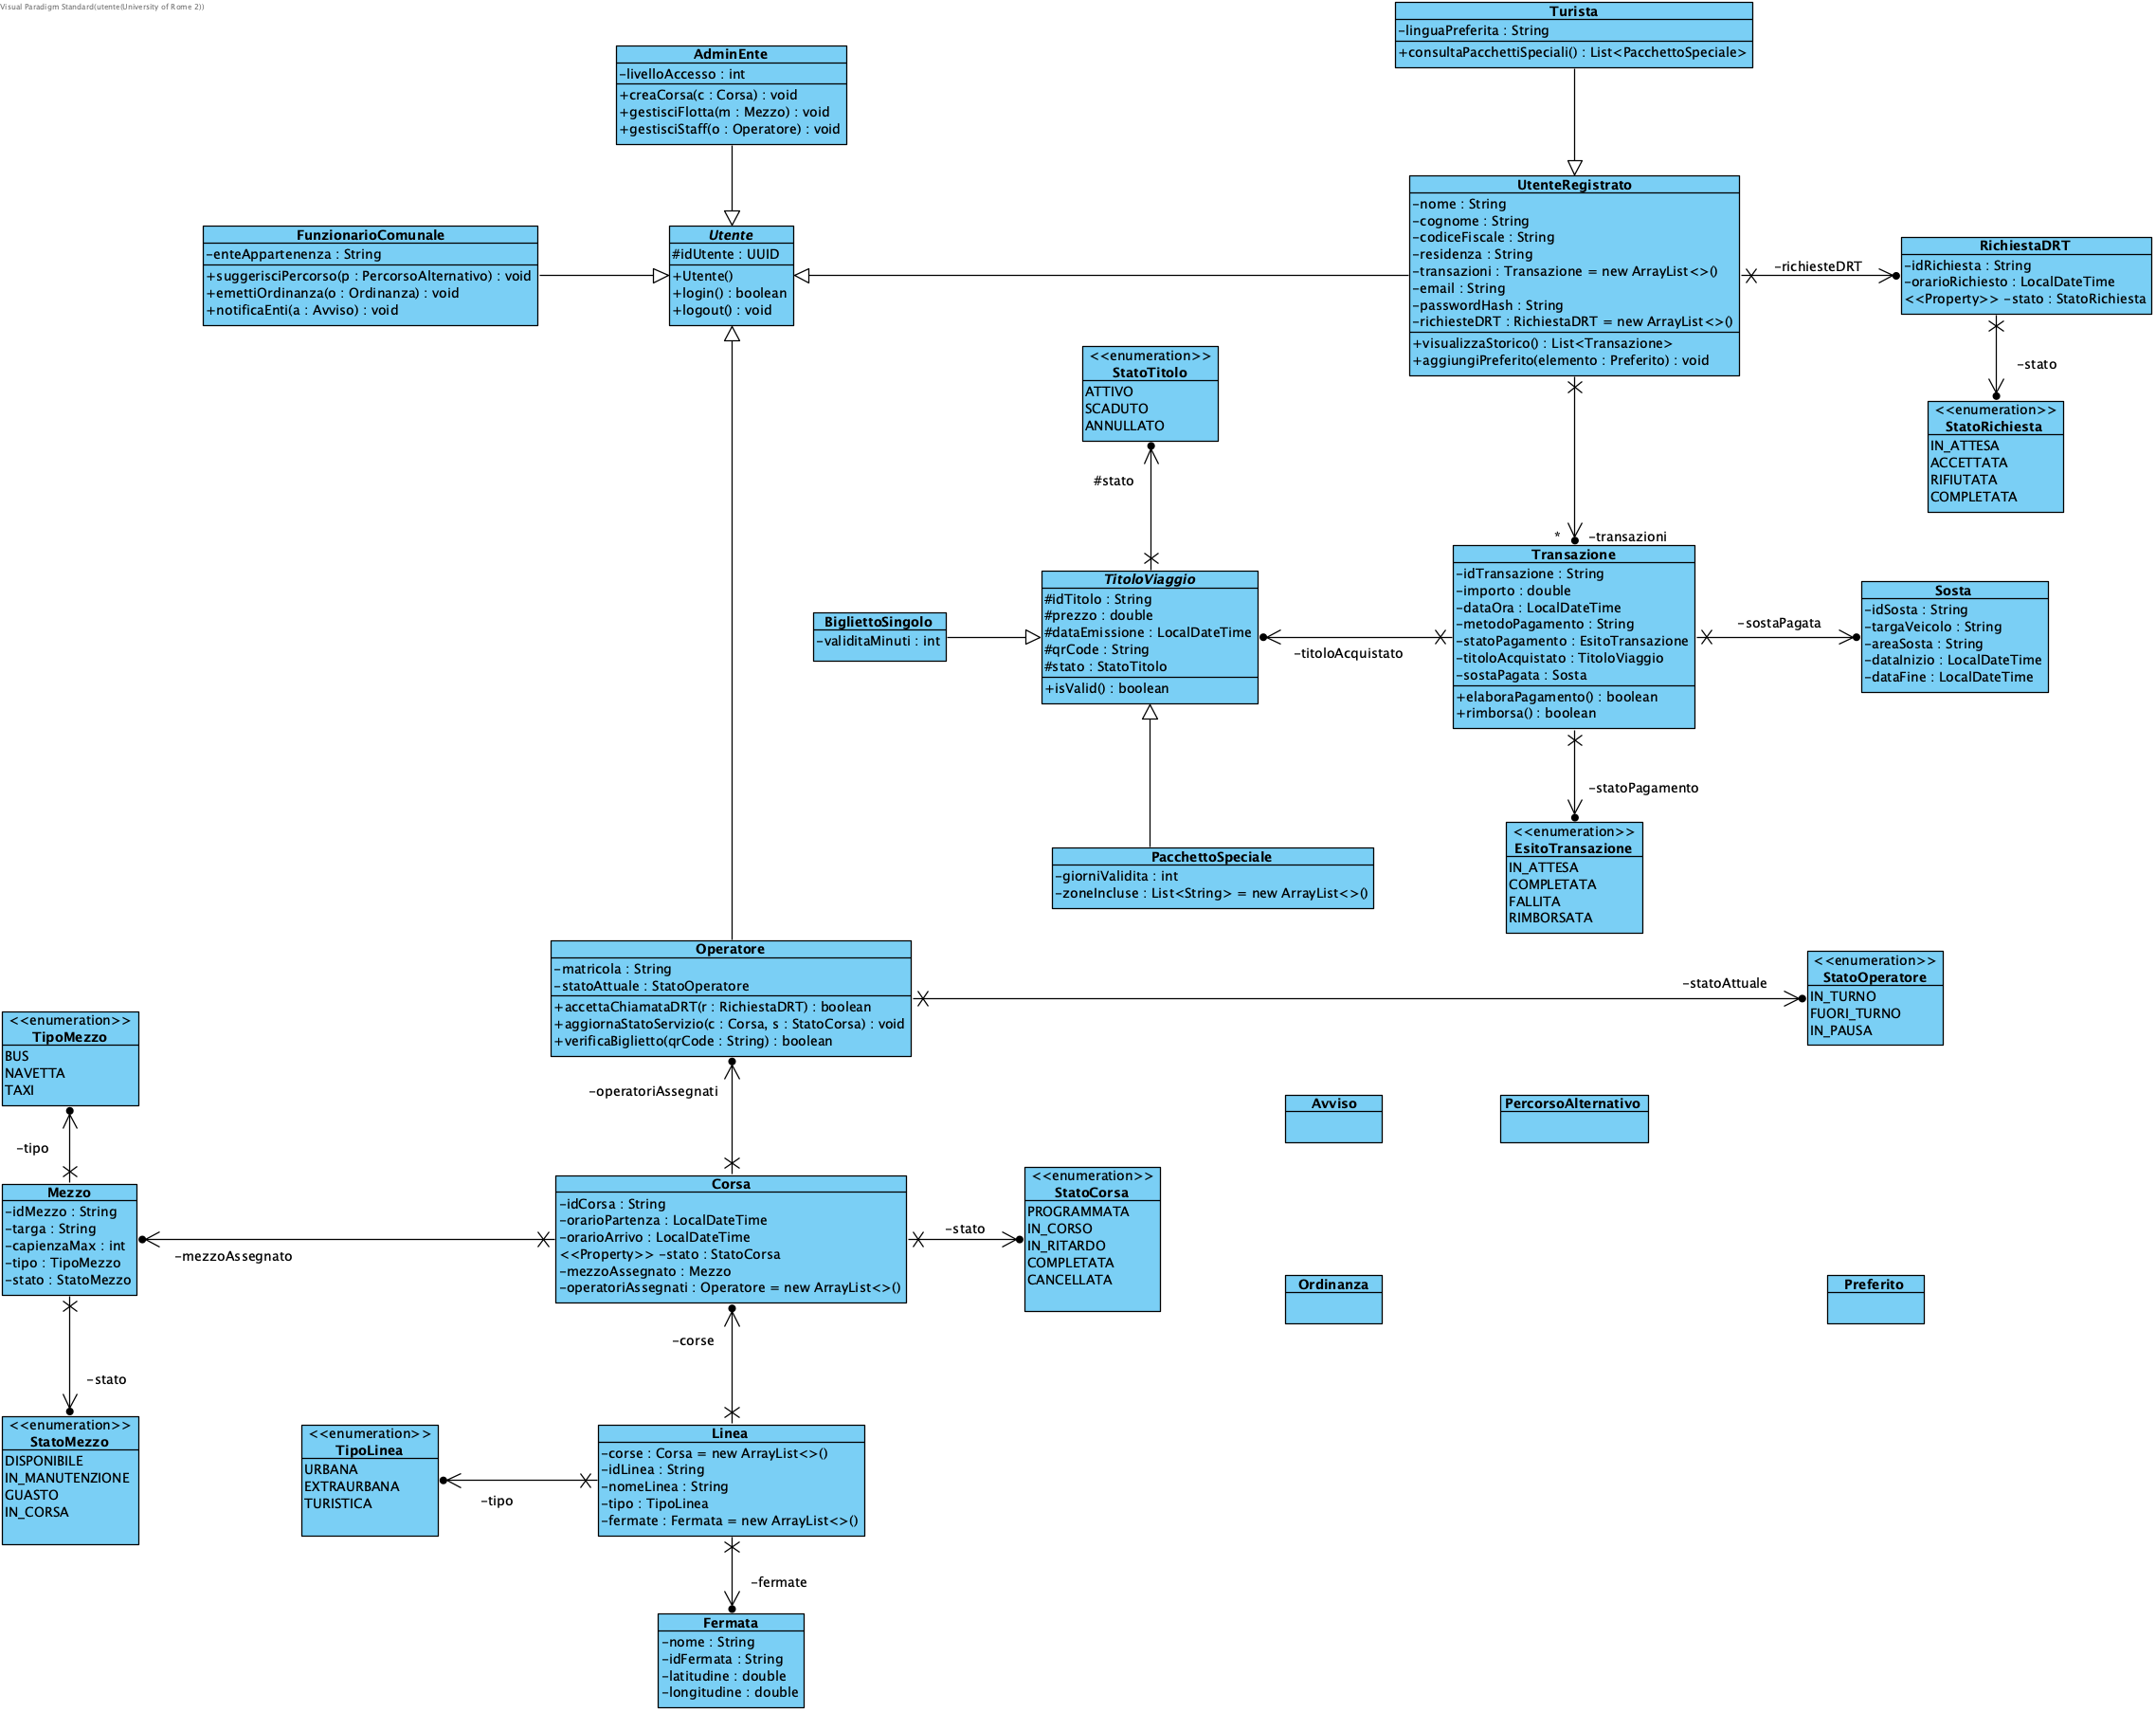
\includegraphics[width=\linewidth]{Class Diagram/Class Diagram4.png}
    \caption{}
    \label{fig:placeholder}
\end{figure}